%% For double-blind review submission, w/o CCS and ACM Reference (max submission space)
\documentclass[sigplan,10pt,review,anonymous]{acmart}
\settopmatter{printfolios=true,printccs=false,printacmref=false}
%% For double-blind review submission, w/ CCS and ACM Reference
%\documentclass[sigplan,review,anonymous]{acmart}\settopmatter{printfolios=true}
%% For single-blind review submission, w/o CCS and ACM Reference (max submission space)
%\documentclass[sigplan,review]{acmart}\settopmatter{printfolios=true,printccs=false,printacmref=false}
%% For single-blind review submission, w/ CCS and ACM Reference
%\documentclass[sigplan,review]{acmart}\settopmatter{printfolios=true}
%% For final camera-ready submission, w/ required CCS and ACM Reference
%\documentclass[sigplan]{acmart}\settopmatter{}

\usepackage{enumitem}
\usepackage{booktabs}
\usepackage{amssymb}
\usepackage{soul}
\usepackage{xspace}
\usepackage{color}
\usepackage{xcolor}
\usepackage{upquote}
\usepackage{listings}
\usepackage{amsmath}
\usepackage{cleveref}
\usepackage{wrapfig}
\usepackage{syntax}

\captionsetup[figure]{font=footnotesize,name={Fig.},labelfont={bf, footnotesize}}
\captionsetup[table]{font=footnotesize,name={Tab.},labelfont={bf, footnotesize}, skip=2pt, aboveskip=2pt}
\captionsetup{font=footnotesize,labelfont={bf, footnotesize}, belowskip=2pt}

\newcommand{\eg}{{\em e.g.}, }
\newcommand{\ie}{{\em i.e.}, }
\newcommand{\etc}{{\em etc.}\xspace}
\newcommand{\vs}{{\em vs.} }
\newcommand{\cmpn}{compartmentalization} 
\newcommand{\heading}[1]{\vspace{4pt}\noindent\textbf{#1}\enspace}
\newcommand{\ttt}[1]{\texttt{\small #1}}
\newcommand{\ttiny}[1]{\texttt{\scriptsize #1}}
\newcommand{\spol}[1]{\scriptsize{\sc#1}}
\newcommand{\pol}[1]{\texttt{\small {\color{purple}#1}}}
\newcommand{\rf}[1]{\ref{#1}}
\newcommand{\wka}{\ttt{a\textsubscript{1}}}
\newcommand{\wkq}{\ttt{q\textsubscript{1-4}}}

% For comments
\newcommand{\eat}[1]{}
\newcommand{\TODO}[1]{\hl{\textbf{TODO:} #1}\xspace}
\newcommand{\todo}[1]{\hl{#1}\xspace}
\newcommand{\nv}[1]{[{\color{cyan}#1 --- Nikos}]}
\newcommand{\kk}[1]{[{\color{magenta}#1 --- kk}]}
\newcommand{\review}[1]{{\color{red}#1}}

\definecolor{editorGray}{rgb}{0.95, 0.95, 0.95}
\definecolor{editorOcher}{rgb}{1, 0.5, 0} % #FF7F00 -> rgb(239, 169, 0)
\definecolor{editorGreen}{rgb}{0, 0.5, 0} % #007C00 -> rgb(0, 124, 0)

\definecolor{cdb}{rgb}{0.37, 0.62, 0.63} % cadet blue

\lstdefinelanguage{sh}{
  morekeywords={for, in, do, done, \|},
  keywordstyle=\color{purple}\ttfamily,
  % ndkeywords={curl, grep, wget, awk, xargs, find, nc, mdc, gunzip, cut, sort, head, join},
  ndkeywordstyle=\color{black}\ttfamily\bfseries,
  identifierstyle=\color{black},
  sensitive=false,
  comment=[l]{\#},
  commentstyle=\color{lightgray},
% morecomment=[s]{/\\*\\*, \\*/},
  stringstyle=\color{darkgray}\ttfamily,
  morestring=[b]',
  morestring=[b]",
% numbersep=1pt,
% numberstyle=\footnotesize\bf\color{gray},   % the style that is used for the line-numbers
  abovecaptionskip=0pt,
  aboveskip=0pt,
  belowcaptionskip=0pt,
  belowskip=0pt,
  frame=none                     % adds a frame around the code
% moredelim=[s][\color{gray}]{c:}{>},
% moredelim=[s][\color{orange}]{/*}{/}
}

\lstset{ %
  backgroundcolor=\color{white},   % choose the background color; you must add \usepackage{color} or \usepackage{xcolor}
  basicstyle=\small\ttfamily,  % the size of the fonts that are used for the code
  upquote=true,
  captionpos=b,                    % sets the caption-position to bottom
% frame=B,                    % adds a frame around the code
  numbers=left,                    % where to put the line-numbers; possible values are (none, left, right)
  numbersep=2pt,                   % how far the line-numbers are from the code
  numberstyle=\tiny\color{gray},   % the style that is used for the line-numbers
  rulecolor=\color{black},         % if not set, the frame-color may be changed on line-breaks within not-black text (e.g. comments (green here))
  framerule=0pt,
	xleftmargin=0pt,
	xrightmargin=0pt,
	breakindent=0pt,
  aboveskip=0pt,
  framesep=0pt,
  abovecaptionskip=0pt,
  aboveskip=0pt,
  belowcaptionskip=0pt,
  belowskip=0pt,
  frame=none,
  framexbottommargin=0pt,
  resetmargins=true
}



%% Conference information
%% Supplied to authors by publisher for camera-ready submission;
%% use defaults for review submission.
\acmConference[PL'18]{ACM SIGPLAN Conference on Programming Languages}{January 01--03, 2018}{New York, NY, USA}
\acmYear{2018}
\acmISBN{} % \acmISBN{978-x-xxxx-xxxx-x/YY/MM}
\acmDOI{} % \acmDOI{10.1145/nnnnnnn.nnnnnnn}
\startPage{1}

%% Copyright information
%% Supplied to authors (based on authors' rights management selection;
%% see authors.acm.org) by publisher for camera-ready submission;
%% use 'none' for review submission.
\setcopyright{none}
%\setcopyright{acmcopyright}
%\setcopyright{acmlicensed}
%\setcopyright{rightsretained}
%\copyrightyear{2018}           %% If different from \acmYear

%% Bibliography style
\bibliographystyle{ACM-Reference-Format}
%% Citation style
%\citestyle{acmauthoryear}  %% For author/year citations
%\citestyle{acmnumeric}     %% For numeric citations
%\setcitestyle{nosort}      %% With 'acmnumeric', to disable automatic
                            %% sorting of references within a single citation;
                            %% e.g., \cite{Smith99,Carpenter05,Baker12}
                            %% rendered as [14,5,2] rather than [2,5,14].
%\setcitesyle{nocompress}   %% With 'acmnumeric', to disable automatic
                            %% compression of sequential references within a
                            %% single citation;
                            %% e.g., \cite{Baker12,Baker14,Baker16}
                            %% rendered as [2,3,4] rather than [2-4].


%%%%%%%%%%%%%%%%%%%%%%%%%%%%%%%%%%%%%%%%%%%%%%%%%%%%%%%%%%%%%%%%%%%%%%
%% Note: Authors migrating a paper from traditional SIGPLAN
%% proceedings format to PACMPL format must update the
%% '\documentclass' and topmatter commands above; see
%% 'acmart-pacmpl-template.tex'.
%%%%%%%%%%%%%%%%%%%%%%%%%%%%%%%%%%%%%%%%%%%%%%%%%%%%%%%%%%%%%%%%%%%%%%


%% Some recommended packages.
\usepackage{booktabs}   %% For formal tables:
                        %% http://ctan.org/pkg/booktabs
\usepackage{subcaption} %% For complex figures with subfigures/subcaptions
                        %% http://ctan.org/pkg/subcaption


\begin{document}

%% Title information
\title{Distribution-oblivious Programming with Dish}         %% [Short Title] is optional;
% \titlenote{with title note}             %% \titlenote is optional;
%                                         %% can be repeated if necessary;
%                                         %% contents suppressed with 'anonymous'
% \subtitle{Subtitle}                     %% \subtitle is optional
% \subtitlenote{with subtitle note}       %% \subtitlenote is optional;
                                        %% can be repeated if necessary;
                                        %% contents suppressed with 'anonymous'


%% Author information
%% Contents and number of authors suppressed with 'anonymous'.
%% Each author should be introduced by \author, followed by
%% \authornote (optional), \orcid (optional), \affiliation, and
%% \email.
%% An author may have multiple affiliations and/or emails; repeat the
%% appropriate command.
%% Many elements are not rendered, but should be provided for metadata
%% extraction tools.

%% Author with single affiliation.
\author{First1 Last1}
\authornote{with author1 note}          %% \authornote is optional;
                                        %% can be repeated if necessary
\orcid{nnnn-nnnn-nnnn-nnnn}             %% \orcid is optional
\affiliation{
  \position{Position1}
  \department{Department1}              %% \department is recommended
  \institution{Institution1}            %% \institution is required
  \streetaddress{Street1 Address1}
  \city{City1}
  \state{State1}
  \postcode{Post-Code1}
  \country{Country1}                    %% \country is recommended
}
\email{first1.last1@inst1.edu}          %% \email is recommended

%% Author with two affiliations and emails.
\author{First2 Last2}
\authornote{with author2 note}          %% \authornote is optional;
                                        %% can be repeated if necessary
\orcid{nnnn-nnnn-nnnn-nnnn}             %% \orcid is optional
\affiliation{
  \position{Position2a}
  \department{Department2a}             %% \department is recommended
  \institution{Institution2a}           %% \institution is required
  \streetaddress{Street2a Address2a}
  \city{City2a}
  \state{State2a}
  \postcode{Post-Code2a}
  \country{Country2a}                   %% \country is recommended
}
\email{first2.last2@inst2a.com}         %% \email is recommended
\affiliation{
  \position{Position2b}
  \department{Department2b}             %% \department is recommended
  \institution{Institution2b}           %% \institution is required
  \streetaddress{Street3b Address2b}
  \city{City2b}
  \state{State2b}
  \postcode{Post-Code2b}
  \country{Country2b}                   %% \country is recommended
}
\email{first2.last2@inst2b.org}         %% \email is recommended

\newcommand{\cf}[1]{(\emph{Cf}.\S\ref{#1})}
\newcommand{\sx}[1]{(\S\ref{#1})}
\newcommand{\sys}{{\scshape Dish}\xspace}
\newcommand{\unix}{{\scshape Unix}\xspace}

\setlist{noitemsep,leftmargin=10pt,topsep=2pt,parsep=2pt,partopsep=2pt}

%% Abstract
%% Note: \begin{abstract}...\end{abstract} environment must come
%% before \maketitle command
\begin{abstract}
  \nv{placeholder}
  Distributed systems offer notable benefits over centralized ones.
  Reaping these benefits, however, requires programming in a way that makes distribution explicit---\eg via new programming languages, distributed framework interfaces, or distribution annotations.
% 
%   \emph{Distribution-oblivious programming} is a new approach for..?
  This paper presents \sys, a shell variant that automatically and correctly scales out distribution-oblivious shell pipelines. %  with regards to the sequential program.
  % leveraging the insight that such programs already express stream computations, with their stages falling under a few, known distributability classes.
  \sys's insight is that shell pipelines already express stream computations that can automatically distributed.
  To achieve this, \sys
% a series of techniques for automatically 
decomposes primitives into distributability classes,
identifies high-distributability stages,
applies rewriting rules for largest possible subprograms,
and orchestrates the distributed program.
Its runtime component provides orchestration and planning support during the execution of the program.
% 
% Key challenges include 
% surprisingly expressive, 
% maximally distributable subprograms
% 
Experiments for complex pipelines show substantial speedups and the ability to operate on large input datasets, all without any developer input.
\end{abstract}


%% 2012 ACM Computing Classification System (CSS) concepts
%% Generate at 'http://dl.acm.org/ccs/ccs.cfm'.
\begin{CCSXML}
<ccs2012>
<concept>
<concept_id>10011007.10011006.10011008</concept_id>
<concept_desc>Software and its engineering~General programming languages</concept_desc>
<concept_significance>500</concept_significance>
</concept>
<concept>
<concept_id>10003456.10003457.10003521.10003525</concept_id>
<concept_desc>Social and professional topics~History of programming languages</concept_desc>
<concept_significance>300</concept_significance>
</concept>
</ccs2012>
\end{CCSXML}

\ccsdesc[500]{Software and its engineering~General programming languages}
\ccsdesc[300]{Social and professional topics~History of programming languages}
%% End of generated code


%% Keywords
%% comma separated list
% \keywords{keyword1, keyword2, keyword3}  %% \keywords are mandatory in final camera-ready submission


%% \maketitle
%% Note: \maketitle command must come after title commands, author
%% commands, abstract environment, Computing Classification System
%% environment and commands, and keywords command.
\maketitle


\section{Introduction}
\label{intro}

\kk{The title is too abstract and doesn't really hint that we
  distribute shell code. Also we could consider capitalizing the name
  as DiSh?}

% 1. Shell scripting; pipelines, in particular, are a common abstraction for expressing filters
% They are an easy way to , because they combine a set of assumptions that work well with Unix
% They work great on a single machine, but are difficult to scale out
% Could we fully automate distribution? 
% The key insight is that pipelines already express a domain-specific
% computation that is easily amenable to distribution.
% 

Distributed systems offer significant benefits over their centralized counterparts---for example, they can speed up expensive computations or can process data that would not fit into any single machine.
% offer notable benefits over their centralized counterparts:
%   using partitioning and replication, they can process and store data with increased throughput and fault-tolerance.
% Yet, only a minority of developers, employed by the select few companies that deal with massive datasets, have the luxury of engineering software systems with distribution baked in from the start.
% The remaining majority starts by developing and deploying software in a centralized manner---that is, \emph{until} there is a significant change of requirements, such as a load increase.
Despite these benefits, their development remains different from and significantly more difficult than their centralized counterparts.
Whereas anyone can quickly stitch together a Bash script to compute on a single computer, 
  % domain-experts routinely glue scripts together to process and share data. % without the help of a computing expert.
   scaling out to multiple ones requires expert labor around ``point'' solutions with expensive setups, restricted programming interfaces, and exorbitant composition costs~\cite{taurus:14, dios:13, andromeda:15, pywren:17, futuredata:18, nefele:18}.

To understand this sharp contrast, consider a Bash pipeline calculating term frequencies over a set of inputs:

% \begin{lstlisting}[language=sh,float=h,numbers=none]
% cat doc.ms |                   # print input file
% groff -t -e -mandoc -Tascii |  # remove formatting
% col -bx |                      # remove backspaces 
% tr A-Z a-z |                   # convert to lower case
% tr -d '[:punct:]' |            # remove punctuation
% sort |                         # put words in alphabetical order
% unique |                       # remove duplicate words
% comm -13 /usr/share/dict -     # report words not in dictionary 
% \end{lstlisting}

\begin{lstlisting}[language=sh, float=h, numbers=none, escapeinside={($}{$)}]
cat * | tr -cs A-Za-z\n | tr A-Z a-z |    ($$[p_1]$$)
  sort | uniq -c | sort -rn | head 5 > out
\end{lstlisting}

\noindent
Program $p_1$ creates a character stream, breaks it into words, transliterates to lower-case, sorts to group duplicates, reduces duplicates to a counter, sorts counters in descending order, picks the top five results, and writes them to a file \ttt{out}.
Combining several features, \unix makes small tasks easy to express;
  for a user with \emph{one} computer and small input size, this pipeline takes a few seconds to compose and execute~\cite{bentley1986literate}.
% composition allows the composition of general primitives

% Key insight 
% % The garden-hose philosophy is similar to Haskell 
% This pipeline takes an input file (line 1), removes 
% * do not need to use specialized frameworks for composition---instead, as long as they conform to the shell, individual primitives can be written in any programming language.
% * do not need to rewrite ---

\begin{figure}[t]
\centering
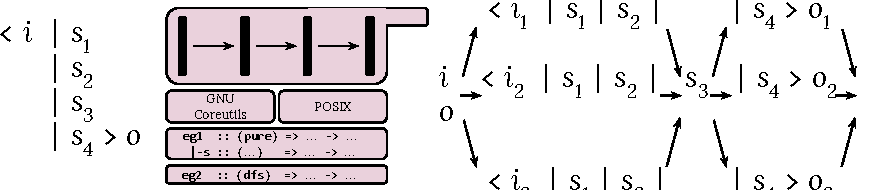
\includegraphics[width=0.49\textwidth]{\detokenize{./figs/dish_schematic.pdf}}
\caption{
  \textbf{\sys high-level schematic.}
	\sys XYZ
}
\label{fig:schematic}
\end{figure}


%      dish      ignis, mozart    hadoop, spark, ...      erlang, elixir
%       \/           \   /             \     /                \   /
% auto <-------------------------------------------------------------> manual
%                      [rewrite (not write) cost]

Unfortunately, developing $p_1$'s distributed equivalent requires a significant effort.
% For a user with many computers and larger inputs, 
% The scope of such rewrites, and therefore the cost of manual effort, can vary considerably.
For simple pipelines, fitting into restricted models of computation, this effort amounts to expressing the computation using the primitives provided by a big-data framework~\cite{mapreduce:08, ciel:11, spark:12, naiad:13} or domain-specific language~\cite{alvaro2011consistency, distal:13, meiklejohn2015lasp}---an unjustifiable cost for one-off pipelines that take a few minutes to compose (but are applied to large datasets).
More complex pipelines, such as the ones presented in later sections, would involve a full-fledged distributed programming language~\cite{erlang:96, lopes1997d, acute:05, mace:07, cloudhaskell:11, ScalaLoci:18}. %  or a distributed operating system---\eg Plan9's \ttt{rc} shell.
In both cases, manual rewriting is expensive and can introduce new bugs, cascading changes, and divergence from legacy functionality.
Could the generation and execution of $p_1$'s distributed version be fully and correctly automated?

% Some (parts of) pipelines require only moderate effort, as they are 
% For some pipelines, this effort is merely moderate, as 
%  can be expressed in domain-specific frameworks---for example, Hadoop and Spark provide a few purely functional primitives that 
%   ---still requiring rewriting the program in a different (\eg Scala for Spark).
% 
% This effort is moderate if the program expressed by these pipelines fits into a domain-specific framework.
% At times, such pipelines
% As long as the program fits into the model this is only moderately difficult;
% 
% For many legacy pipelines  
%  has to choose between three options, all of which require significant manual effort.
% The most invasive is to rewrite the entire program in a distributed programming language
% The most popular is to leverage 
% 
% Use a distributed programming language, even higher rewrites
% Or use some form of annotations 
% 
%  this requires rewriting portions of the program in a new language and use operations
% 
% 
% In the simplest case, annotations
% 
% Often, they only focus on a few parts of the system---for example, upgrading to a distributed storage layer.
% More rarely, companies rewrite entire systems (\eg Twitter's Ruby-to-Scala rewrite~\cite{twitter}), a process that is notoriously difficult under schedule constraints and competitive pressures~\cite{rewrite1, rewrite2}.
%  especially since software today makes extensive use of third-party modules~\cite{breakapp:plos:2017}.
% 

% If developers have already expressed their computation as a Unix pipeline, they should not have to manually rewrite the program in other environment---\eg Hadoop, Spark---to exploit distribution.


To answer this question, this paper presents \sys, a shell \todo{preprocessor} that transforms shell pipelines into their distributed equivalents enabling \emph{distribution-oblivious programming}.
The key insight behind \sys is that the language of the Unix shell already encodes stream processing, providing most of the information required to distribute a computation\kk{I am not sure whether stream processing provides information for distributing a computation on its own. Maybe we can say that the shell exposes operator level parallelism, and that this is the first step to distributing a computation}.
\sys builds on this insight with a careful study of the distributability properties of shell primitives and commands, a pipeline rewriting pass that identifies \todo{maximal} sub-expressions as candidates for scale-out, and a late-bound command-prefixing scheme for deferring scheduling decisions to the distributed planner (\ie when runtime information is available).
A \sys-enabled $p_1$ will run \ttt{tr} and \ttt{uniq} in completely parallel streams \kk{Isn't uniq pure? I am not sure how we can handle it}, use a mostly-parallel tree of \ttt{sort}s, run \ttt{head} in one of the streams, and (trivially) merge streams in \ttt{out}.

The combination of automated transformations for program distribution with the ability to maintain correct non-distributed semantics results in several benefits.
% \sys converts legacy shell pipelines into their distributed equivalents fully automatically, offering $100\times$ improvements in performance without a single line of additional code or annotation.
First, shell users composing pipelines (or simply running legacy pipelines on massive datasets) can see scalability benefits without any manual effort---no need for \ttt{qsub}~\cite{gentzsch2001sun}, \textsc{SLURM}~\cite{yoo2003slurm}, calls to \textsc{GNU} \ttt{parallel}~\cite{Tange2011a}, or any manual rewriting~\cite{mapreduce:08, ciel:11, spark:12}.
Second, developers of new shell commands can use a concise a domain-specific language to express their distributability properties rather than using ad-hoc, command-specific flags such as {\tt -t},  {\tt NUM\_THREADS}, \ttt{-t}, \ttt{-p} \etc
Most importantly, \sys provides an architectural lesson for system designers---namely, that large-scale research efforts in the distributed- and operating-system literature to provide a \unix-like distributed equivalent~\cite{ousterhout1988sprite, mullender1990amoeba, pike1990plan9, barak1998mosix} would have been simplified by a thin (but sophisticated) rewriting shim like the one \sys provides.
% Nice critique on parallel: https://bugs.debian.org/cgi-bin/bugreport.cgi?bug=597050#75

% % Make Unix benefits explicit?
% Indeed, the primary reason behind $p_1$'s succinctness is that the pipeline is a domain-specific language for describing operations over streams.
% Key elements of \unix are the ability to compose programs written in different languages, the abstraction of a file system as a set of resident streams, a small but extensible library of commands, and the ability to resolve names within a global context.
% Under the hood, the \unix kernel buffers results, synchronizes processing stages, and generally orchestrates the computation.

% Primitives 
% \sys enables \emph{distribution-oblivious programming}: 
%   multi-order of magnitude speedups with correctness guarantees and without any developer effort.
% 
% The a series of transformations that 
% Second, we are using describing composition . For this, we are restricting the study to a subset of the POSIX shell--
% 
% Local operations and identifiers have to be carefully translated to distributed ones, a translation that depends on the types of the operations and associated identifiers.
% 
% The semantics is enough to capture powerful features such as stream branching and feedback constructs found in practice and in the system's evaluation.

The paper is structured as follows.
It first starts with a background section outlining pipeline concepts and overviewing \sys~\sx{bg}.
Sections \ref{classes}--\ref{recipes} highlight key contributions:\footnote{
  This is not precise, we'll need to wait until it matures a bit.
}
\begin{itemize}

  \item
  \S\ref{classes} overviews \sys and introduces several scalability and distributability classes.

  \item
  \S\ref{rewrite} presents a set of rewriting transformations for identifying maximal pipeline sub-expressions, candidates for scale-out.

  \item
  \S\ref{other} details other concerns, such as distributed state management and extensibility.
\end{itemize}

\noindent
\sys's evaluation~\sx{eval} shows significant speedups on both parallel and distributed execution, using a combination of micro-bench\-marks---popular shell one-liners that highlight certain features---and multi-line macro-benchmarks---a web crawling and indexing engine, a genomics pipeline, and a popular weather analysis script.
After a comparison with related prior work~\sx{related}, the paper closes with a discussion of related work and possible future directions~\sx{discussion}.

% \begin{figure*}[t]
% \centering
% 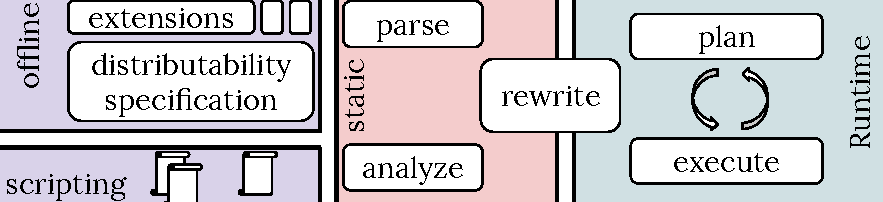
\includegraphics[width=0.49\textwidth]{\detokenize{./figs/dish_overview.pdf}}
% \caption{
%   \textbf{Applying \sys to $p_1$.}
% }
% \label{fig:example}
% \end{figure*}
% 

\section{Background}
\label{bg}

This section breaks down $p_1$ to presents important background on and challenges
of shell scripting.

\subsection{Unix Composition, Informally}
\label{bg:pipelines}

% A pipeline is a mechanism for program composition that works by chaining together programs (or, \emph{commands}) using pipes.
\unix provides several ways for succinct program composition.
Central among them is the \emph{pipe}, a primitive that passes the output of one program as input to the next.
These programs produce output and consume input concurrently, and possibly at different rates, with the \unix kernel facilitating program scheduling and communication synchronization behind the scenes.
Intermediate programs, termed commands, can also be developed in different programming languages, as long as they conform to a common interface.
\begin{wrapfigure}{r}{0.06\textwidth}
  \vspace{-12pt}
  % \begin{center}
    % \includegraphics[width=0.48\textwidth]{gull}
    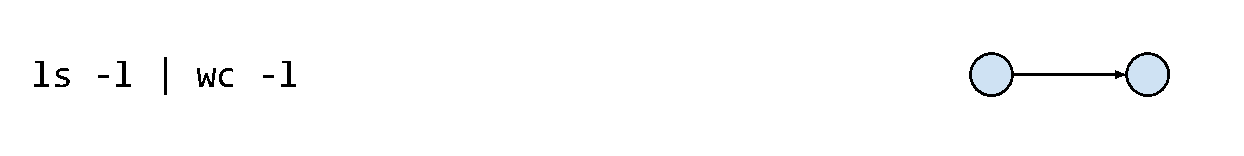
\includegraphics[width=0.06\textwidth]{\detokenize{./figs/dish_ex1.pdf}}
  % \end{center}
  \vspace{-30pt}
\end{wrapfigure}
This interface exposes a stream of contiguous character lines.
A few characters are special---for example, the newline (\textsc{NL}) character delineates an element of the stream, and the end-of-file (\textsc{EOF}) character signals the end of a stream.
As part of this interface, each command has access to (any combination of) three \emph{standard} streams---input, output, and error.
% the input stream (stdin), the output stream (stdout), and the generating errors or diagnostics to the standard error stream (stderr)
% generating errors or diagnostics to the standard 
% Leveraging this interface, pipelines chain together commands by their standard streams, such that the output stream of one command (stdout) is passed directly as input (stdin) to the next one.
% TODO: \kk{We have to mention character vs line based parallelism somewhere, and that we choose to see lines as the data quantum}

Commands can be tuned by two mechanisms, namely command-line options and environment variables.
Options control the execution of a program---\eg changing the \ttt{sort}ing order.
The shell does not have any visibility into these options; 
  their parsing and evaluation is left entirely up to each command \kk{A minor point: the shell does the expansion, and then hands it of to the command (I am saying that because evaluation might be confounded with expansion so we might want to clarify that)}.
Environment variables carry more general information about the surrounding system---\eg file search paths, system defaults, parsing switches \etc 
They are organized in a map from names to values, both of which are strings, and can be evaluated at any point in the program---including as commands, flags, a shell feature termed parameter \emph{expansion}.

% TODO: Talk about security primitives?
Streams are a key feature of \unix, and go hand-in-hand with the file abstraction:
  files are simply persistent streams that can be manipulated by commands or pipelines.
\begin{wrapfigure}{r}{0.15\textwidth}
  \vspace{-15pt}
  % \begin{center}
    % \includegraphics[width=0.48\textwidth]{gull}
    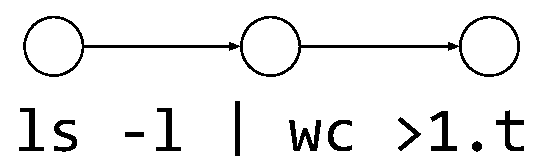
\includegraphics[width=0.15\textwidth]{\detokenize{./figs/dish_ex3.pdf}}
  % \end{center}
  \vspace{-25pt}
\end{wrapfigure}
Reading a file or a set of files generates a stream; 
  similarly, streams can be trivially redirected to the file system---by appending with the file identifier.
Files are named, in the sense that they correspond to a global identifier---for example \ttt{cat /x/y} returns the persistent stream associated with the identifier \ttt{/x/y}.
\unix exposes a few different types of files---\eg directories, symbolic links, named pipes (or FIFOs), and special character devices.
As a result, file-system identifiers part of a pipeline may resolve to in-memory structures or pseudo-devices (\eg \ttt{/dev/urandom}).

% At a high level, POSIX defines several file types:
% (-) regular files, storing lines of text or binary data,
% (d) directories, grouping together multiple other files,
% (l) symbolic links, pointing to other files,
% (p) named pipes or FIFOs, communication primitives that can be named and manipulated like files,
% (s) domain sockets or DSes, full-duplex communication primitives that support passing file descriptors, and
% (b or c) special files, interfaces to device drivers or low-level abstractions, presented as ordinary files.

Special files are particularly interesting because they are resolved to OS structures.
One example is the special \ttt{/proc} filesystem (procfs) that presents information about processes and the operating system, offering a feature analogous to programmatic introspection:
  with \ttt{procfs} commands can inspect and alter their directory or the flags passed to them.
% Here are a few examples:
% (i) \ttt{/proc/PID/cmdline} contains the command that originally started the process,
% (ii) \ttt{/proc/modules} contains a list of the kernel modules currently loaded, and
% (iii) \ttt{/proc/PID/cwd} contains a symlink to the current working directory of the process.
Similarly, \unix exposes file-system handles for various ephemeral structures, including standard streams.
This bidirectional relationship between ephemeral streams and persistent names---the fact that streams can be named in the file-system and files can be converted to streams---is a key enabler of the runtime rebinding achieved during our transformations.

A small but powerful set of features is concerned with stream manipulation.
Some of these features are built into the shell;
  for example, given a file identifier, stream redirection operators can direct stdout or stderr to a file.
\begin{wrapfigure}{r}{0.15\textwidth}
  \vspace{-15pt}
  % \begin{center}
    % \includegraphics[width=0.48\textwidth]{gull}
    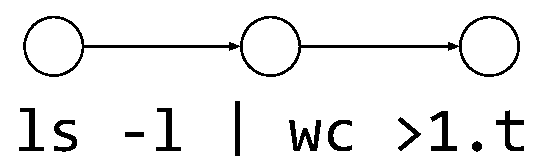
\includegraphics[width=0.15\textwidth]{\detokenize{./figs/dish_ex3.pdf}}
  % \end{center}
  \vspace{-25pt}
\end{wrapfigure}
As described before, the file can be a FIFO dubbing as input to another command.
More interestingly, some commands allow splitting (resp. merging) a single stream (resp. many streams) into multiple streams (resp. a single stream);
  stream merging can be achieved by appending one stream after the end of another or by fusing (zipping) streams column-wise into a single (fat) stream.
% TODO: talk about \ttt{xargs}?

% Explicit Redirection, Implicit splitting and merging, This can be done through the file-system operators 

The combination of file-system identifiers pointing to ephemeral streams and the stream redirection described above enable surprisingly expressive pipelines. %---for example:
The most interesting feature of these pipelines is the presence of cycles:
  a pipeline segment processes some input, part of which is extracting the next input to process.
One example use case, discussed in the evaluation section~\sx{eval} is a web crawler that feeds extracted URLs from the input stream back to the start of the pipeline.
% These streams are created by the C library (glibc) at the start of program execution,
% and new streams can be created to connect to files, sockets, pipes,

Apart from pipes, the \unix shell provides several other forms of program composition such as sequential (\ttt{;}) and parallel (\ttt{\&}) composition operators.
Command substitution, expressed as \ttt{\$($c$)}, replaces the expression with the results of executing $c$.
Code blocks, expressed as \ttt{\{$c_1; c_2$\}}, can redirect streams for the entire group of $c_1$ and $c_2$;
  this is analogous to an anonymous function, which contains many statements and can possibly be assigned to a variable that can later be invoked with parameters.
Subshells, enclosed in \ttt{($c_1; c_2$)}, are similar to code blocks but spawn a child shell, thus avoiding the pollution of their environment variable context. % but incurring higher overhead.


% \begin{lstlisting}[
%   language=es,
%   mathescape,
%   float=t,
%   belowskip=-5mm,
%   label=core-pl,
%   upquote=true,
%   caption={
%     \textbf{The core language of the POSIX shell.}
%     The language used by ; file identifiers and expansion are not shown.
%   }]
% $p$ ::= $s\in{}String$ | $n\in{}Number$ | $b\in{}Bool$ | $\emptyset$
% $v$ ::= $p$ | ($x$,$\ldots$) => {e} | {$s$:$v$,$\ldots$} | [$v$,$\ldots$]
% $e$ ::= x | $v$ | ($x$ = $e$) $e$ | $e$($e$) | $e$[$e$] = $e$
% \end{lstlisting}

% \begin{lstlisting}[language=sh, float=h, numbers=none, escapeinside={($}{$)}]
%  cat /proc/ >                            (($$p_4$$))
% \end{lstlisting}
% \begin{lstlisting}[language=sh, float=h, numbers=none, escapeinside={($}{$)}]
%  ls -l | wc -l                           (($$p_2$$))
% \end{lstlisting}
% \begin{lstlisting}[language=sh, float=h, numbers=none, escapeinside={($}{$)}]
%  cat * | wc -l > out.txt                 (($$p_3$$))
% \end{lstlisting}
% \begin{lstlisting}[language=sh, float=h, numbers=none, escapeinside={($}{$)}]
%  cat /proc/ >                            (($$p_5$$))
% \end{lstlisting}
% \begin{lstlisting}[language=sh, float=h, numbers=none, escapeinside={($}{$)}]
% { echo 1; echo 2; } > out.txt
% \end{lstlisting}

\begin{figure}[t]
\centering
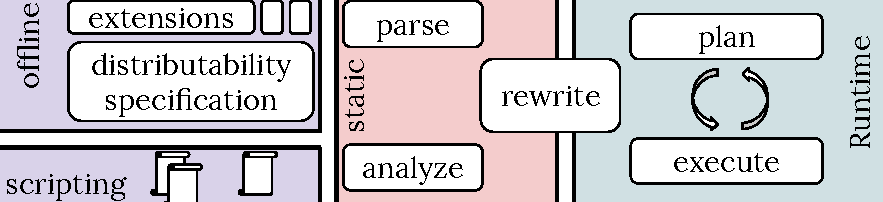
\includegraphics[width=0.49\textwidth]{\detokenize{./figs/dish_overview.pdf}}
\caption{
  \textbf{\sys transformation overview.}
	\sys XYZ
}
\label{fig:overview}
\end{figure}


% \heading{Generation}
% Expansion---the key is that expansion and evaluation are handled by the shell at an earlier stage 
% The most powerful---and interesting, for \ttt{dish}---type of expansion is subshell expansion, that allows replacing entire input streams 

\subsection{Overview}

As outlined earlier, the key insight behind \sys is that the shell already describes parallel computations over streams.
Intuitively,
 (i) the parallel-composition operator exposes \todo{task} parallelism \kk{I have named that operator level parallelism, which one do we prefer?},
 (ii) commands such as \ttt{xargs} and \ttt{tee} expose data parallelism,
 (iii) the pipe operator enables both task and data parallelism, and \kk{How does it enable data parallelism?}
 (iv)  other composition operators can be viewed as barrier candidates.
To leverage these insights and correctly distribute a pipeline such as $p_1$, \sys must solve several challenges.

Understanding the shell's primitives is not enough;
  \sys has to understand the distribution characteristics of individual commands used to compose larger programs.
This challenge can be broken down into two parts.
First, there is a need to understand the commands already in the shell---that is, built-ins that come with any shell and support its core functions.
One example is the set of commands defined by the \textsc{POSIX} standard~\cite{}.
\sys addresses this part by a careful study of a group of commands, identifying a small but clear set of well-understood distributability classes.
This set is already useful enough to allow the composition of practical pipelines~\sx{eval}.

The second part is expressing such characteristics extensions that fall outside the built-in set, allowing new commands to leverage \sys's power.
Commands are arbitrary programs, but still conform to the shell's pipeline interface.
To solve this part, \sys leverages the prior study to define a small but expressive domain-specific language (DSL) for describing a command's key properties with respect to its distributability.
Using this DSL, developers of commands (not users of the shell) can quickly and easily capture the class of the command.
A command developer can only annotate the default behavior;
  if a new flag is added a few years later, and if that flag alters the command's class, only then a new annotation is needed.

Given a set of commands composed together by the shell primitives, \sys's next challenge is to analyze it and identify candidate subexpressions for distribution.
\sys addresses this challenge with a rewriting \todo{pass} that performs dataflow analysis identifying \todo{maximal} distributable sub-expressions.
It converts the AST to a dataflow graph, and runs...
This analysis is not trivial, as many of the shell's dynamic features have to be taken into consideration---examples include shell expansion, environment variables, file input sizes, \etc

\kk{On the dataflow graph, Dish iteratively performs graph transformations that expose data parallelism as task parallelism while preserving correctness.}

Finally, given a distributed pipeline with runtime \todo{annotations}\kk{the runtime just gets a dataflow graph}, \sys needs to schedule and execute it.
This amounts to solving a few challenges, achieved by \sys's runtime component, two of which stand out.
First, \sys needs to wrap single-node commands with corrective runtime interposition based on their classes;
  this is achieved by thin wrappers for all the commands involved in the program, generated just-in-time using the distributability specification outlined earlier.
The reasoning behind wrappers being thin is to not interfere with legacy functionality---commands have many flags accumulated over long periods of time.

Second, \sys needs to fill-in planing details left blank by the rewriting pass.
This is achieved with \emph{planner activators}, commands that yield (and pass their arguments) to the scheduler.
From the point of view of the shell, activators are higher-order commands \'{a} la \ttt{xargs} and \ttt{time} that take other commands as arguments---a technique that achieves the latest possible binding, when critical runtime information is available. \kk{I am not exactly sure I understand that :) }

The next few sections discuss the details.
They also outline other, less obvious challenges---such as the synchronization of environment variables, distributed file operation, \etc.


\section{Distributability Classes}

\subsection{Comnands}
\label{bg:cmd}

% Sets vs. Classes

\begin{table}[h]
\center
\footnotesize
\setlength\tabcolsep{3pt}
\caption{
  \footnotesize{
    \textbf{Distributability Classes}.
    Broadly, \unix commands can be broken down into to five classses.
  }
}
\begin{tabular}{l @{\extracolsep{\fill}} lll}
\toprule
Class                           & Example Commands        & POSIX            & Core-utils\\
\midrule
Stateless                       &                         &                  &           \\
Pure                            &                         &                  &           \\
(Distr.) File-System            &                         &                  &           \\
Side-effectful                  &                         &                  &           \\
Irreversibly Side-effectful     &                         &                  &           \\
% \midrule
% Shell PL Constructs             &                         &                  \\
% \etc                            &                         &                  \\
\bottomrule
\end{tabular}
\label{tab:classes}
\end{table}


Define distributability 
Explain distributability classes, based on how 

\heading{Preliminaries}

\heading{POSIX, GNU Core-utils, and beyond}

\heading{Stateless}

\heading{Pure}

\heading{File-system}

\heading{Side-effectful}

\heading{Irreversably Side-effectful}

\subsection{The Shell Language}
\label{bg:shell}

\heading{Implicits}
Expansion
Implicits
Context

\heading{Language Constructs}

Even without these, the Unix pipeline language is powerful enough to capture complex pipelines.

We can encode powerful

\section{Dish Overview}


\section{Extensibility}
\label{ext}

Here is the type for \ttt{bwa}, a command that performs a Burrows-Wheeler transform over genomic data:
% ( bwa ) :: ( Pure )  => { In \/ File* } -> { Out /\ Err }    -- default case
%    | -h :: ( Sless ) => { Out }                              -- if needed
\begin{lstlisting}[language=sh, float=h, numbers=none, escapeinside={($}{$)}]
(bwa) :: (Pure) ($$\Rightarrow$$){In($$\lor$$)File*}($$\rightarrow$$){Out($$\land$$)Err}
  |-h :: (Sless)($$\Rightarrow$$){Out}                              
\end{lstlisting}

It states that the command defaults to the Pure class.
It's operation can be thought as a transformation from input streams to output streams.
It operates either on stdin or, if this doesn't exist, one or more files specified as arguments;
% TODO: check actual man page for how to specify files
  it writes to the output and error stream rather than a file.
The \ttt{-h} flag moves \ttt{bwa} into the Stateless class;
  its output is a constant function.


ULTRA DRAFTY:

\kk{Text point: A problem that is specific to the shell is
  extensibility.}

The major characteristic that makes the shell popular and very useful
is its extensibility, as also mentioned in \Cref{bg}. Commands change,
get extended, and each user continuously installs more commands to use
in their system.

\kk{Text point: This restricts the space of solutions for distribution
  of shell scripts}

This means that any one-time solution is not satisfactory, since it
would very easily become obsolete, or it would only handle a limited
amount of shell scripts.

\kk{Text point: The characteristics of a good solution}

A solution that applies to shell programms should thus be extensible,
in the sense that adding or changing a command, doesn't invalidate the
assumptions that the tool makes. In our case, the information about
the command categories. A developer of a new command, should be able
to categorize it accordingly, and succinctly describe how the system
can distribute a command.

\kk{Solution: A lightweight language that can be used by a command
  developer to categorize it for distribution.}

We address this issue by designing a lightweight language whose
purpose is to categorize a command, describes how it reads its input
(meaning in what order), and how to distribute it (in case it is
pure). \kk{I am not sure if the order in which a command reads its
  input will be part of the language since many commands can be made
  to read from one place (like stdin or their first argument). Even in
  that case though, where the command only reads from one argument, we
  have to make sure that there is a way for the user to pinpoint which
  argument does a command read from.}

\subsection{Categorization Language}

\kk{Text point: Introduce problem: Most shell commands, belong to
  different classes depending on their flags, arguments}

Consider the command \texttt{cat} \kk{Maybe that is not he best
  example. TODO: Find a good example of a simple command that is in
  different classes depending on the arguments.}. When used without
any flag it is stateless, etc...

\kk{Text point: Our language must be able to categorize commands to
  different classes according to their arguments.}

\kk{We should have a crisp point about why we have this categorization
  language, and why don't we just allow someone to write a function in
  python for each command, that given the command and its arguments,
  returns whether the command category. Possible arguments include,
  the fact that this language is simpler to use, especially by non
  experts that just run some script but have installed some commands
  that are not ``supported''. Another possible argument is that we
  could be able to reason about the constructs of the categorization
  lagnauge, and that they will be easier to read and
  understand. Another argument is that since these categorizations
  should be shareable among users, it would be bad to execute
  arbitrary python code, so using this language, expressivity is
  limited. All of these arguments are a little bit weak though. Niko,
  what do you think?}

\kk{New sketch of the language}

We assume that commands satisfy the standard that options and flags
come first, and then file arguments. The language contains a record
for each command name, together with a sequence of predicates that map
to command categories and designation of input output.

%% Can be tricked according to this:
%% https://tex.stackexchange.com/questions/24886/which-package-can-be-used-to-write-bnf-grammars

\begin{grammar}
  <flag> ::= `-' <string>

  <category> ::= `stateless' | `pure' | ...

  <arg> ::= `arg[' <int> `]'

  <input> ::= `stdin' | <arg>

  <output> ::= `stdout' | <arg>

  <flag-pred> ::= <flag>
  \alt `value' <flag> = <string>
  \alt `!' <flag-pred>
  \alt <flag-pred> `or' <flag-pred>
  \alt <flag-pred> `and' <flag-pred>

  <assignment> ::= `(' <category>, <input>, <output> `)'

  <predicate> ::= <flag-pred> `=>' <assignment>

  <pred-list> ::= `|' <predicate> <pred-list>
  \alt `|' `otherwise' `=>' <assignment>

  <command> ::= <name> `:' <pred-list>

\end{grammar}

\kk{We don't need to designate the stderror, because we assume that it
  is never the main output of a command and it will never be used by
  the input of another command in the pipeline. If someone indeed
  wants to do this, they can just use a redirect I think to get around
  it.}

\kk{Give an example of a flag that has value and how this could alter
  category or input etc...}



Sketch of the language:

Some kind of lightweight annotation configuration language (like
yaml), that contains a record for each command.

A record contains a sequence of predicates => categories. Each
predicate is a combination of not, or, and and the atomic predicates
are the presence of a flag, or an equality that checks that the value
of a flag is equal to something (because flags can also have
values). The final predicate can be left empty, and it is trivially true.

Interpreter:

Given a command and the set of its arguments, the intepreter returns
the command category. In does so by returning the category of the first
predicate that matches.

\kk{Would it be meaningful to give the syntaxx of the language
  formally?}

\kk{If we talk about the language it would be good to give some
  statistics about how many commands (out of the ones that we have
  classified) can be represented with one, two clauses etc. If we have
  a different solution (like python function that given a command and
  its arguments returns the category) then we could talk about how
  many lines of code it took to categorize all the commands that we
  did.}

As described in distributability\ref{}, the abstract notion of a
program that we have is programs with one input and one output
stream. The command developer must be able to express the input
argument of a commmand (or if it is the stdin).

\kk{Question: Do we need to handle all commands (even the ones that
  could have their input split in several different arguments? or can
  we somehow easily make these ones just take their input from one
  place (e.g. by adding a cat before them).}

\kk{Possible solutions for this (if we have already turned commands
  with more that one input to commands with one input): Have a
  positional reference to the argument that is input (or ``stdin'' if
  it is the stdin). Example: the last argument [-1] of grep is its
  input.}

\kk{It seems that even the arguments might depend on flags (e.g. grep
  checks the current directory if asked recursively, or the stdin
  otherwise), so maybe we should again have a sequence of predicates}


\kk{Note: Since a categorization language will probably not be
  complete (especially the one showing the input arguments) there
  should be a backup mechanism, when the language is not expressive
  enough, like a python function that categorizes the command, and
  returns its input argument if it is stateless.}

\subsection{Pure Commands}

Even though stateless commands are a big percentage of all of them,
there are a lot of useful and popular pure commands.

As mentioned in distributability, pure commands can be broken down
into different categories. We might be able to get ideas about this
from this paper:
\url{http://www.cs.toronto.edu/~azadeh/papers/pldi17-ex.pdf} and its
continuation in PLDI 2019.

\kk{Can we find a solution for the commands in coreutils?}

\kk{Important TODO: Find at least one more command that can be
  executed like sort. Does wc work? If there is no pure command that
  can be easily parallelized other than sort, this story is not very
  nice.}



\section{Dataflow Graph Model}
\label{ir}

\TODO{Replace texttt with inline listings?}

In order to effectively apply optimizations and distribute a shell
script, it first has to be translated to a manipulable
representation. As mentioned in \ref{}, the two main abstractions of
the shell, are files that contain data, and commands that communicate
through these files. We propose a slight variation of the standard
dataflow graph model, that is commonly found in stream processing
systems, as the representation of a distributed shell computation. The
main benefit of the dataflow graph model is that it clearly exposes
task parallelism, as different nodes can be independent processing
workers. In our case each node represents a command, and each edge
represents a file.

\subsection{Graph Components}

\paragraph{Nodes - Commands}

Nodes $f$ of the graph represent functions from one (possibly empty)
input stream to an output stream $f : D^* \rightarrow D^*$. $D$
represents the basic data type of a line of characters. This
representation captures the majority of shell commands. The nodes are
monotonic, meaning that they cannot retract their output. More
formally, $\forall f, x, y, f(x) = y$, then for any $x'$, there exists
$y'$ such that $f(x.x') = y.y'$, where $.$ is standard concatenation
and will be omitted when obvious. An example of a node is the
following command \kk{Does it need ref? Also maybe this example is too
  trivial and can be removed.}:

\begin{lstlisting}[language=sh, float=h, numbers=none, escapeinside={($}{$)}]
 grep ``foo''
\end{lstlisting}

\noindent
This command takes a stream of lines from its standard input and
returns a stream of lines on its standard output. An important
observation is that commands in the shell might read their input
stream from a sequence of different sources. An illustrative example
is the command \texttt{cat} which reads its input from a combination
of files and its standard input.

\begin{lstlisting}[language=sh, float=h, numbers=none, escapeinside={($}{$)}]
 cat x - y
\end{lstlisting}

The example above reads file \texttt{x} until it encounters the EOF
character, then reads from \texttt{stdin}, and then reads from
\texttt{y}. In order to handle this particularity, nodes in the
dataflow graph can have many incoming edges, that are ordered in a
sequence. Note that this does not correspond to standard dataflow
graph representations where the semantics of multiple incoming edges
is either zipping the inputs in pairs, or arbitraliy interleaving them.

\TODO{Is the following paragraph best suited here? It describes an
  assumption that we make about commands, to guarantee the validity of
  our transformations. The assumption is needed due to the limitation
  of the programming model of one input one output per command.}

Note that nodes can read from more files than just the files of their
stream (or respectively write to more files that their output stream),
however these files are static (e.g. used for configuration or logging
\kk{Would an example here help}) and do not represent streams of data,
and therefore are not considered part of the dataflow graph. We assume
that these static files can only be accessed by one node, thus
ensuring that they do not interfere with the distributed
implementation.
%% Because of the assumption in section Front End \ref{}, that each file
%% exists only once in the dataflow graph, we can safely assume that
%% reading and writing to these static files does not interfere with the
%% distributed implementation, and doesn't alter the behaviour of the
%% program.

\paragraph{Edges - Files}

Edges in the dataflow graph represent files, the basic data
abstraction of the shell. They are used as communication channels
between nodes in the graph, and as the input or output of the whole
graph. Edges are represented as possibly unbounded streams of type
$D*$. They could either refer to a specific named file in the file
system, or just be FIFO pipes that used for interprocess communication
\TODO{Are there any other file types, such as URLs, ...?}.

\TODO{Show an example pipe and its graph}.

In order to expose data parallelism from the output of a command,
files that don't point to a resource can have an upper bound on the
lines that they can tranfer. The following example illustrates why
this is essential.

\TODO{Add an example of a command that has two outputs and one goes to
  one command, while another output goes to a different one. Maybe
  only show the graph here and not the command itself.}

On the other hand, some forms of data parallelism can be exposed when
knowing the size of the input files. As mentioned in \ref{} some pure
commands (such as cat -n) only need line information to become
stateless, and knowing the size of a file could allow the system to
split it in different chunks that can be processed independently. To
account for that, edges that refer to an input resource contain the
number of lines of the file that they refer to.

Finally, the edges that don't refer to a resource and do not start
from a node in the graph represent the graph input, while the edges
that don't refer to a resource and do not point to a node in the graph
are its outputs.

\kk{(Maybe) It might be beneficial to mention that many inputs do not
  represent the same thing as many outputs. These two notions are not
  symmetric.}


\subsection{Graph transformations}
\label{ir:transformations}

As mentioned above, the dataflow graph exposes task
parallelism. Different nodes in the graph can be executed
concurrently, communicating through the edges. Task level parallelism
is already exposed by the shell, by using pipes \texttt{|} and the
background operator \texttt{\&}. Unfortunately, simple task
parallelism leaves a lot to be desired, since scaling a computation
requires manually introducing more operators.

In order to adequately utilize the available computational resources,
a distributed implementation should exploit data parallelism. Data
parallelism is based on the observation that some operations produce
the same result when performed independently on subsets of the input
data, merging the results afterwards. This is the basic optimization
that is used by popular distributed processing systems such as
MapReduce\kk{cite} and Apache Spark\kk{cite}. \todo{Unfortunately, the
  dataflow graph model of most of these systems is not expressive
  enough to represent data parallelism, so the distributed generations
  that they generate, can not be represented in their dataflow model.}
\kk{This last sentence is extremely important and we should make it
  shine.}

In contrast, our dataflow model inherently supports the data
parallelism that is found in shell programs. More precisely, data
parallelism can be easily exposed as task parallelism in our model. A
very important consequence of this is that we can iteratively apply
optimizations that expose data parallelism, or even revert them when
the resulting dataflow graph is too wide. This flexibility enables
unified reasoning and implementation of the unoptimized and optimized
version of the dataflow graph. \kk{This is exciting, and maybe it
  should be moved up (or rephrased in the introduction)}

Before describing the different types of parallelization
optimizations, we formalize our intuition about stateless and pure
commands. Recall the example \ref{} from section Categories
\ref{}. This example shows the stateless command x being applied to
...\kk{Complete this after we have an example}. Formally, a commmand
$f$ is stateless if it is ``linear'' with respect to concatenation,
i.e. the following equation holds:

\[
\forall x, x', f(x.x') = f(x).f(x')
\]

Similarly, every pure command $f$ that can be written as a map $m$ and a
reduce $r$ step satisfies the following:

\[
\forall x, x', f(x.x') = r(m(x).m(x'))
\]

Based on these equations, we can define a maximal node split operation
on a stateless node $v$ with $n$ input ordered edges and an output
edge to node $v'$, to replace $v$ with $n$ new nodes, giving each one
of them one of the incoming edges of $v$, and routing them in order to
point to $v'$. The maximal node split operation can similarly extended
for pure nodes.

\kk{If there is time I can work out a formal definition and a proof
  sketch why this transformation preserves the output of the dataflow
  graph}.

%% \begin{definition}
%% Given a dataflow graph $G = (V, E, O)$, where $V$ is a set of nodes
%% representing commands, $E$ is a set of edges representing files, and
%% $O$ is a function from $V \cup v_{out}$ to a total order of incoming
%% edges. $v_{out}$ represents a concatenation of all the outputs of the
%% dataflow graph. We represent the total order for a node $v$ as
%% $<_v$. Given a node a node $v$
%% with input edges $ie = \{ i_1 = (v_{i_1}, v, 1), i_2, ..., i_n =
%% (v_{i_n}, v, n) \}$ and output edge $o = (v, v_o, a)$, we define a
%% complete node split $s(v, G) = (V', E')$ where $V' = V - v \cup \{
%% v_1, ..., v_n \}$ and $E' = E - ie \cup \{(v_{i_1}, v_1, 1), ...,
%% (v_{i_n}, v_n, 1) \} - o \cup \{ (v_1, v_o\}$
%% \end{definition}

%% \begin{lemma}
%% tofill
%% \end{lemma}

In addition to node splits, we can also perform edge splits in order
to increase the number of incoming edges for some nodes to expose
possible data parallelism. If the edge refers to a real file, then the
edge split represents splitting the real file in chunks, while in
cases where the edge connects two nodes, it is split to several edges
with a bounded number of lines. Note that the final output edge of a
valid node in the graph must always be unbounded if it does not refer
to a file.


\kk{Remember to mention the assumptions that need to hold for the
  graph transformations to be valid in the Command categories
  section. Commands must be deterministic, they must not do any other
  side effect (such as writing to other files, sending signals,
  etc). However, these assumptions must already be checked when the
  developer designates the categories.}



\section{Front End}

\kk{The writing in this section is wandering around without a clear
  purpose :( }

\kk{It might make sense to merge this section with the one below with
  the name: From Shell to IR and back}

As mentioned in \Cref{ir}, in order to generate the distributed
implementation of a shell script, \texttt{Dish} first translates it to
a dataflow graph. However, there are several components in shell
programs that cannot be arbitrarily parallelized without affecting the
program behaviour, e.g. commands producing an irreversible effect, or
commands connected with a \texttt{\&\&} operator. In addition, the
fact that the shell is \todo{extremely dynamic}, further increases the
challenge of correctly identifying what parts can be distributed.

%% \kk{Give examples of writing to environment variables, producing
%%   irreversible side effects, the ; and \&\& operators.}

In order to address this issue, we introduce the notion of
distributable program regions, and we design a translation pass that
given the abstract syntax tree of a shell script identifies
distributable regions and translates each of them to a dataflow
graph. The AST of the shell script is produced using a POSIX compliant
parser \kk{Reference libdash github. This las sentence should probably
  go to evaluation}.

\subsection{Distributable Regions}

%% \kk{I wanted this to be purely about the regions, and a next
%%   subsection be about the analysis, but the separation line is very
%%   blurry, so they are now in the same subsection.}

\kk{The goal of this subsection is to explain that Dish does a safe
  but effective analysis to identify which parts of the scripts to
  parallelize.}

Consider the following example:

\begin{lstlisting}[language=sh, float=h, numbers=none, escapeinside={($}{$)}]
  cat f1 f2 | grep ``foo'' > f3 &&
  sort f3 # Replace with sth better
\end{lstlisting}

Notice that the structure of a shell program clearly identifies
components that can be executed concurrently, and barriers that
enforce synchronization. More precisely, \texttt{cat f1 f2} and
\texttt{grep ``foo''} would already execute concurrently in the
standard shell, while \texttt{sort f3} waits for their completion
before being executed. Both \texttt{cat f1 f2 | grep ``foo'' > f3} and
\texttt{sort f3} are maximal distributable regions, in the sense that
they cannot be extended beyond \texttt{\&\&}.

Concretely, a distributable region cannot permeate through the
following barrier constructs: ;, \&\&, \texttt{||}, function
definitions, command substitutions, and control flow primitives. On
the other hand, the pipe operator \texttt{|} and the parallel
composition operator \& enable parallelization, and extend
distributable regions. Essentially, distributed regions correspond to
subsections of the program that would be executed by different shell
processes.

\kk{I don't know whether I should mention the following: While these
  control flow constructs can be parallelized and there has been
  research on it, it is orthogonal to our work, and can be
  incorporated as future work.}

\subsection{Translation Pass}

Dish performs a depth first search pass on the AST of the given shell
program, extending the distributable regions from the bottom up,
translating their independent components to dataflow graph
nodes, until a barrier construct is reached. Note that barrier
constructs can be contained in a dataflow graph, as long as they don't
extend beyong a single node. An illustrative example follows:

\begin{lstlisting}[language=sh, float=h, numbers=none, escapeinside={($}{$)}]
  (sort f1 > g1 && sort f2 > g2) &
  sort -m g1 g2
\end{lstlisting}

In the above example\kk{Can we make example not floating?}, while
\texttt{sort f1 > g1}, \texttt{sort f2 > g2}, and \texttt{sort -m g1
  g2} are all in different dataflow graphs. The dataflow graph that
corresponds to the whole program, has two nodes, \texttt{sort f1 > g1
  \&\& sort f2 > g2} and \texttt{sort -m g1 g2}.

In order to identify possible opportunities for parallelism, the
translation pass also identifies the category of each node, together
with its input and output, using the rules described in \ref{}. Some
interesting cases of the analysis algorithm are shown in pseudocode
below:

\begin{lstlisting}[language=python, float=h]
  def translate(node):
    ...
    elif(node.name == 'Pipe'):
      return pipe_graphs([translate(child)
        for child in node.children])
    elif(node.name == 'And'):
      node.children = [translate(child)
        for child in node.children]
      return node
    elif(node.name == 'Command'):
      if(not safe(node)):
        return make_ir_node(node, 'unsafe')
      else:
        return make_ir_node(node,
          find_category(node))
    ...
\end{lstlisting}

%% \kk{Explain how the three above cases work, mentioning what does
%%   pipe-graphs and safe do. The important point to get across is to
%%   explain why we do the ``conservative checks'' in safe, and how they
%%   preserve safety.}

Whenever the algorithm encounters a pipe node, it recursively
translates its subcomponents, and then merges them in a dataflow graph
by connecting the output of the first with the input of the second,
\etc. Before the different dataflow graphs are connected, the
algorithm checks that at most one node in the graph writes at every
file, and at most one node reads from a file that another node writes
to. This is important, in order to avoid inconsistent behaviour after
distributing nodes in the dataflow graph \kk{Does this need an
  example?}. Whenever the algorithm encounter an \texttt{\&\&} node,
it recursively translates its subcomponents (similarly to the pipe
node), but then doesn't merge them in a large dataflow graph. Finally,
whenever the algorithm encounters a command, it first checks whether
it is safe to possibly parallelize this command. A command is
considered to be safe, if it does not make any modification to the
shell state (e.g. changing the current directory, modifying
environment variables), and if it does not read from a
\todo{read-once} file, like a fifo pipe. \kk{Mention: Note that an
  unsafe command can still be safely added to the dataflow graph as a
  single node, since this doesn't introduce any new
  behaviours. However it cannot be parallelized further than that.} If
the command is considered safe, its category is identified and a node
containing that command is created and added to a singleton dataflow
graph.

It is important to note that due to the highly dynamic nature of the
shell, the safety properties that were mentioned above cannot be
soundly checked statically. For example in the first case, two
unexpaned strings could refer to the same file, but the translation
pass cannot infer that. Hence, in both cases, the checks were
approximated using a \todo{best-effort} method. \kk{Maybe mention that
  as future work, we want to tighly integrate with the shell shtepper
  that will allow to maximally expand everything before making this
  decision.}


\paragraph{Assumptions}

\kk{This paragraph is not extremely necessary. Maybe it can be moved
  to limitations?}

There are two additional assumptions that have to be satisfied in
order for the distributed implementation that is generated by Dish to
have equivalent behaviour with the original implementation. First of
all, there should be no external signals to the commands while they
execute. At the moment Dish assumes no faults, and that communication
always succeeds. This assumption can be lifted by extending Dish with
a fault-tolerant runtime, \kk{blah blah}. Second, we assume that no
command reads and writes to arbitrary files that are not mentioned in
their arguments. This is a necessary assumption, since commands are
considered as black boxes and the only information that can be
inferred about them is through their arguments.


\section{Dish Implementation}

\kk{I think that this section should be merged with the front end}


\paragraph{Dish Optimizer}

The \texttt{Dish} optimizer is given a dataflow graph representing a
shell program and outputs an optimized dataflow graph, where data
parallelism opportunities have been exploited. More concretely, the
optimizer starts by splitting input files in several chunks, given the
desirable output dataflow graph width. It then starts from the source
nodes of the graph, iteratively performing the graph transformations
that were described in \Cref{ir:transformations}. If the incoming
edges of the node are less than the desirable graph width, it performs
edge splits, and then it performs maximal node splits. The final graph
can then be implemented by spawning a process for each node, and
redirecting the outputs according to the graph edges.

\kk{Maybe give an example}


%% \subsection{Mapping operators to nodes}

%% \kk{I don't think we should mention this.}

%% Explain the simple algorithm that we used to minimize intra node
%% communication, that tries to map contiguous parts of the graph to the
%% same node. We could do this by having an algorithm that minimizes the
%% number of cuts or something.

%% We don't try to make a proper planner, as there is a lot of work on
%% operator placement etc. that we can borrow from.

\subsection{Just in time planning}

\TODO{Rename this section to planner activators and write it after I
  discuss with Nikos.}

\kk{This whole section for just in itme planning, is also relevant for
  the front end. If the front end is executed just in time, it would
  have more information, and maybe it could make a sound analysis.}

Important point: Shell is extremely dynamic. Because of this, a
distributor cannot decide how to distribute a subexpression
statically, by just reading the script, (as in many other systems like
MapReduce, Spark, etc), since most of the information is not there
before the script starts executing. Environment variables,
unexpanded(unevaluated) strings \kk{Make sure that terminology is
  consistent with Greenberg}, could all contain information that is
valuable to make the distribution plan \kk{give an example}.


Future work on this: calling the shell shtepper to only partially
evaluate strings, just expand arguments, and not do any significant
computation. Even better, we could be calling the shtepper just after
having parsed the ast, and decide on maximal distributable subtrees as
late as possible in the process. This would be awesome.

\subsection{Merge and Split Implementation}

\TODO{Niko, could you make this a bit stronger?}

It is common in the dataflow graph for a node to have many incoming
edges, or many outgoing edges (when all but the last outgoing edges
are bounded). However some nodes, might only read their input from one
source (e.g. stdin). In this case, the distributed implementation
needs to concatenate input files (or conversely split output
files). Here is an example:

\kk{Show an example graph! of cat | tr | sort. The command in the
  middle must only take input from one file (maybe just stdin).}

We address this issue using primitive shell constructs for file
manipulation. More concretely a merger can be implemented by a simple
\verb|cat|. Given a set of input files \verb|in1, in2, ...| and an
output file \verb|out|, a merger can be implemented as:

\begin{lstlisting}[language=sh, float=h, numbers=none]
 cat $in1 $in2 ... > $out
\end{lstlisting}

\noindent
\TODO{Change that with the new splitter}
On the other hand, given an input file \verb|in| that is a FIFO pipe,
and two output files \verb|out1, out2| the first of which is bounded
to \verb|N| lines, a 2-splitter can be implemented as:

\begin{lstlisting}[language=sh, float=h, numbers=none]
 head -n $N $in > $out1 ; cat $in > $out2
\end{lstlisting}

\noindent
Using the 2-splitter as a building block, a pipe can be split to
arbitrarily many different pipes.


\section{Evaluation}

\kk{We should make sure to measure the time that it takes for the
  whole process to run (parsing, translating, optimizing, planning)
  together with the scripts. This will probably be negligible, but we
  still have to mention it. }

\kk{Also, we have to have one-two handcrafted examples that have more
  than one pipeline, to show the execution time end to end, as this
  cannot be shown with the one-pipeline examples since they only have
  one graph, so no back and forth between shell and dish.}

\kk{Furthermore it would be great to have one distributed example that
  runs in more than one node (if we have time)}

\kk{Also we have to make sure to measure with and without the final
  cat of output file, so that we show that this is also negligible.}

\kk{We have to make sure that we repeat that the results are the same
  in all tests that we run. Corectness, blah blah ...}

\kk{We should have at least some pipelines that have a bad pure
  command in them.}

\section{Limitations}

\kk{This is not really a section on its own, but rather part of something else.}

\begin{itemize}
\item Fault Tolerance
\item Distributed Planning: The planner at the moment is naive, and
  there is a huge literature on operator placement of distributed
  dataflow graphs that can be used to improve it.
\item Support of shell constructs: At the moment we have been
  conservative in the shell subsets that we handle, so that we don't
  introduce any unsafe parallelism. The point of this work was not to
  be able to handle a complete distributable subset of the shell, but
  rather a significantly big part of it, to demonstrate that there can
  be performance benefit from it.
\item Support distributing different classes: At the moment we are
  only dealing with stateless and pure commands, that is the ones that
  are most popular but also can offer the biggest benefits from
  parallelizing them. However, it would be interesting to explore the
  distributability of the file system commands, by using a distributed
  file system. THis would also require considerations about
  replication, consistency, and failures.
\item No cycles (multiple commands writing and reading from the same file)
\item Formal proof that the analysis indeed returns distributable
  subtrees. Previously there was no formal semantics for shell, but
  recent work (cite greenberg) allows us to make a formal proof that
  the analysis is indeed sound.
\end{itemize}

\section{Related Work}
\label{related}

\kk{On our dataflow graph model: Our data flow graph model is
  different than most distributed batch and stream processing systems,
  since the shell is a hybrid between the two. Batch processing
  systems have no notion of data order, and stream processing systems
  usually have order, but none of these systems supports this notion
  of reading from different sources in sequence. Our dataflow graph
  model supports this by including information about incoming edge
  order. Another benefit of our dataflow model, is that together with
  the equations that hold on stateless and pure commands, data
  parallelism is exposed in the graph as task parallelism. This allows
  the unoptimized and optimized dataflow graph to have the same
  unified representation, and doesn't lead to an ad-hoc optimization
  of the dataflow graph as done in the other systems (the last bit is
  too aggressive). }

At a high-level, techniques for automatically distributing fall under a spectrum that ranges from fully automated (but potentially sub-optimal) distribution to fully manual (but, ideally, optimal) distribution (Fig.~\ref{fig:spectrum}).

\begin{figure}[t]
\centering
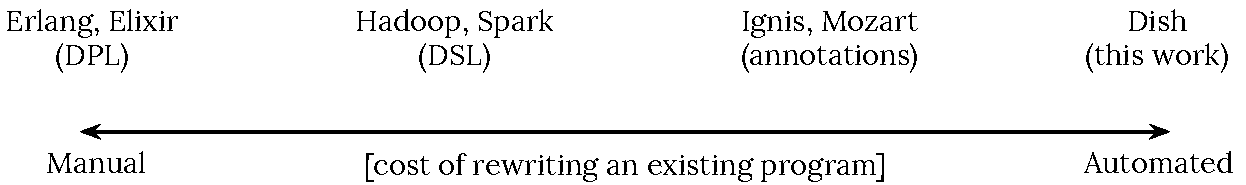
\includegraphics[width=0.49\textwidth]{\detokenize{./figs/dish_spectrum.pdf}}
\caption{
  \textbf{Cost of Manual Effort.}
	\sys sits at the automation end of the spectrum, automatically distributing shell pipelines while maintaining their correctness. A more complete picture is presented in the related-work section~\sx{rt}.
}
\label{fig:spectrum}
\end{figure}

% Nice intro: http://homepages.inf.ed.ac.uk/bfranke/Publications/pldi121-tournavitis.pdf
\heading{Automated Parallelization and Distribution}
There is a long history of automated parallelization starting from explicit \ttt{DOALL} and \ttt{DOACROSS} annotations~\cite{par1, par2} and continuing with compilers that attempt to automatically extract parallelism~\cite{padua1993polaris,hall1996maximizing}.
These systems operate at a lower level than \sys (\eg that of instructions or loops instead of pipe boundaries) and typically do not exploit runtime information.

% https://ecommons.cornell.edu/bitstream/handle/1813/6508/85-668.pdf?sequence=1
% The growth of the web led to specialized frameworks for massively distributed computation~\cite{mapreduce:08, spark:10, naiad:13}.
% While they Moreover, these systems take advantage of functional purity;
%   for programs that are not data-intensive processing pipelines (\eg web servers), purely functional code is generally responsible for only a small fraction of the program runtime.
A plethora of systems assist in the construction of distributed software.
Distributed operating systems~\cite{rashid1981accent, walker1983locus, ousterhout1988sprite, mullender1990amoeba, pike1990plan9, rozier1991overview, dorward1997inferno, barak1998mosix, schwarzkopf2013dios, sacha2013osprey} and programming languages~\cite{erlang:96, acute:05, mace:07, cloudhaskell:11}
% simplify many of the problems of distribution and
provide a significant amount of automation. % but require development in a new system or language.  While they take care of all the distribution minutiae, 
However, they involve significant manual effort using the provided abstractions, which are strongly coupled with the underlying operating or runtime system.
\TODO{This has to be broken down into systems and PLs, coz systems are the most relevant/important class.}

\heading{Annotation-based Distribution}
Ignis and Mozart

\heading{DSLs for Distribution}
At the other end of the spectrum, distributed computing frameworks~\cite{mapreduce:08, ciel:11, spark:12, naiad:13, jetstream:14} \kk{JetStream has a very different focus} and domain-specific languages~\cite{alvaro2011consistency, distal:13, meiklejohn2015lasp, psync:16, dartagnan:18}
simplify certain patterns, 
but do not offer the flexibility of a full-fledged environment.
% suffer from a similar lack of generality by making strong assumptions about the nature of the computation---for example, strongly-eventual commutative components that can proceed in parallel.
Developing under these frameworks differs quite significantly from the development of normal (non-distributed) programs.

More recent work focuses on extracting parallelism from domain-specific programming models~\cite{cilk5, streamIt, galois} and interactive parallelization tools~\cite{parascope, ipat}.
These tools simplify the expression of parallelism, but still require programmers to get involved in discovering and exposing parallelism.
%  actively involve the programmer in the detection and mapping of application parallelism, but still demand great effort from the user. 
Moreover, the insights behind these attempts are significantly different from ours, as they extract parallelism statically during compilation instead of dynamically during runtime.
%Despite significant progress~\cite{}, it remains due to its need for complex program analysis and the unknown factors (such as input data range) during compilation.

\kk{We need to cite DGSH}

\section{Conclusion}
\label{discussion}


\begin{acks}
  % Dumping people so that we don't forget
  % 
  This material is based upon work supported by the
  \grantsponsor{GS100000001}{National Science
    Foundation}{http://dx.doi.org/10.13039/100000001} under Grant
  No.~\grantnum{GS100000001}{nnnnnnn} and Grant
  No.~\grantnum{GS100000001}{mmmmmmm}.  Any opinions, findings, and
  conclusions or recommendations expressed in this material are those
  of the author and do not necessarily reflect the views of the
  National Science Foundation.
\end{acks}


%% Bibliography
\bibliography{./bib}


%% Appendix
\appendix
\section{Scripts used in the evaluation}

This appendix contains the source code of the scripts used in the evaluation of
the \sys. They are part of the codebase (released as open source with the camera
ready), and are provided here only to aid the reviewers.


\end{document}
